\documentclass[11pt]{article}

\usepackage[most]{tcolorbox}
\usepackage{luatexja}
\usepackage{array}
\usepackage[margin=25mm]{geometry}

%セルの長さを指定して縦にそろえる
\newcolumntype{M}[1]{>{\centering\arraybackslash}m{#1}}

\setlength{\parindent}{0pt}
\linespread{1.2} %行間を調整

%tcolorboxのスタイルを設定
\tcbset{
  mybox/.style={
    %colback=yellow!5,
    %colframe=orange!80!black,
    fonttitle=\bfseries,
    title=#1
  }
}

\begin{document}

\begin{tcolorbox}[mybox={直線}]
2点を線で結ぶことを考える。2点を結ぶように両方向に伸ばした線を\textbf{直線}という。\\
2点の間を線で結んだ線を\textbf{線分}という。一方向だけに伸ばした線を\textbf{半直線}という。\\
点$A$と点$B$を通る直線を、\textbf{直線$AB$}と呼ぶ。線分や半直線についても同じ。\\

\begin{tikzpicture}
%直線
\coordinate (P1) at (0,0);
\coordinate (A1) at (1,0);
\coordinate (B1) at (3,0);
\coordinate (Q1) at (4,0);
\draw[thick] (P1)--(Q1);
\fill[blue] (A1) circle (2pt);
\fill[blue] (B1) circle (2pt);
\node[xshift=0pt, below=5pt] at (A1) {A};
\node[xshift=0pt, below=5pt] at (B1) {B};
\node at (2,1) {直線AB};

%線分
\coordinate (A2) at (6,0);
\coordinate (B2) at (9,0);
\draw[thick] (A2)--(B2);
\fill[blue] (A2) circle (2pt);
\fill[blue] (B2) circle (2pt);
\node[xshift=0pt, below=5pt] at (A2) {A};
\node[xshift=0pt, below=5pt] at (B2) {B};
\node at (7.5,1) {線分AB};

%半直線
\coordinate (A3) at (11,0);
\coordinate (B3) at (14,0);
\coordinate (Q3) at (15.5,0);
\draw[thick] (A3)--(Q3);
\fill[blue] (A3) circle (2pt);
\fill[blue] (B3) circle (2pt);
\node[xshift=0pt, below=5pt] at (A3) {A};
\node[xshift=0pt, below=5pt] at (B3) {B};
\node at (12.5,1) {半直線AB};
\end{tikzpicture}
\end{tcolorbox}

\bigskip

点や直線に、アルファベットで名前をつけます。その理由は、、、\\

図の中に点や直線がたくさんあったときに、どの点や直線のことを説明しているか混乱しやすいです。そのため、点や直線に名前を付けることが多いです。名前をつけることで、はっきりと説明ができます。\\

名前としては、A,B,Cなどのアルファベットで名前をつけます。\\
\begin{center}
\begin{tikzpicture}
\coordinate (A) at (1,1);
\node[below=3pt] at (A) {A};
\fill[black] (A) circle (2pt);
\draw[thick] (4,0)--(8,1);
\node at (6,1) {L};
\end{tikzpicture}
\end{center}

%長さが同じ記号と中点
\begin{tcolorbox}[mybox={中点}]
線分の真ん中の点を\textbf{中点}という。\\

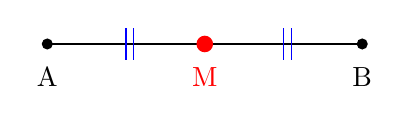
\begin{tikzpicture}
\coordinate (A) at (0,0);
\coordinate (B) at (4,0);
\coordinate (M) at (2,0);
\draw[thick] (A)--(B);
\fill[black] (A) circle (2pt);
\fill[black] (B) circle (2pt);
\fill[red] (M) circle (3pt);
\node[xshift=0pt, below=5pt] at (A) {A};
\node[xshift=0pt, below=5pt] at (B) {B};
\node[xshift=0pt, below=5pt,red] at (M) {M};
%同じ長さの記号
\draw[blue] (1,0.2)--(1,-0.2);
\draw[blue] (1.1,0.2)--(1.1,-0.2);
\draw[blue] (3,0.2)--(3,-0.2);
\draw[blue] (3.1,0.2)--(3.1,-0.2);
\end{tikzpicture}
\end{tcolorbox}

%角をアルファベットで表す
%角度が同じ記号
\begin{tcolorbox}[mybox={角と三角形}]
三角形の各頂点に記号をつけて、三角形の名前を決める。\\
例えば、各頂点にA,B,Cという名前をつけたとき、三角形ABCと呼ぶ。\\
記号では、$\triangle$ABCとかく。
三角形の頂点の記号は反時計回りにつけることが多い。\\

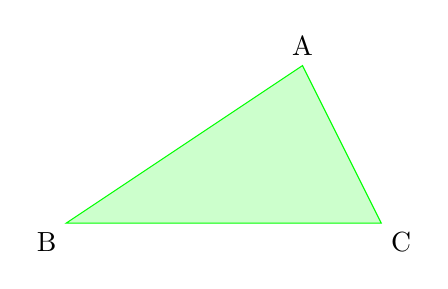
\begin{tikzpicture}
\coordinate (B) at (0,0);
\coordinate (C) at (4,0);
\coordinate (A) at (3,2);
\node[below left] at (B) {B};
\node[below right] at (C) {C};
\node[above] at (A) {A};
\draw[green,fill=green!20!white] (A)--(B)--(C)--cycle;
\end{tikzpicture}
\end{tcolorbox}

%直線の位置関係
\begin{tcolorbox}[mybox={垂直と平行}]
2つの直線が交わらないとき、2つの直線は\textbf{平行}という\\
1つの直線にもう一つの直線が直角に交わるとき、直線は\textbf{垂直}であるという\\
線分に垂直に交わり、中点を通る直線を\textbf{垂直二等分線}という。\\

\begin{tikzpicture}
\draw[thick] (0,-1)--(3,0);
\draw[thick,red] (0,0)--(3,1);
\draw[thick] (5,0)--(9,0);
\draw[thick,blue] (7,1.5)--(7,-1.5);
\draw[blue] (7,0.25)--(7.25,0.25)--(7.25,0);
\end{tikzpicture}
\end{tcolorbox}

\begin{tcolorbox}[mybox={距離}]
\begin{tikzpicture}
\draw[thick] (0,2)--(4,2);
\draw[thick] (0,0)--(4,0);
\draw[red,thick] (2,2)--(2,0);
\draw[red] (2,0.3)--(2.3,0.3)--(2.3,0);
\draw[red] (2,1.7)--(2.3,1.7)--(2.3,2);

\coordinate (P) at (8,2);
\fill[black] (P) circle (2pt);
\draw[thick] (6,0)--(10,0);
\draw[red,thick] (P)--(8,0);
\draw[red] (8,0.3)--(8.3,0.3)--(8.3,0);
\draw[dashed] (P)--(9,0);
\draw[dashed] (P)--(6.5,0);
\end{tikzpicture}
\end{tcolorbox}

%図形の移動
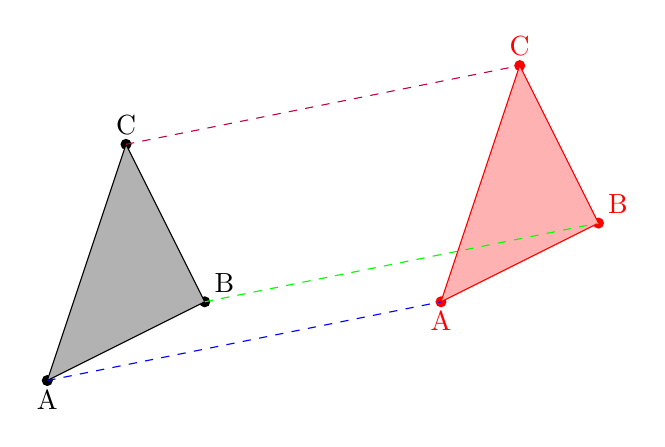
\begin{tikzpicture}
\coordinate (A1) at (0,0);
\coordinate (B1) at (2,1);
\coordinate (C1) at (1,3);

\coordinate (A2) at (5,1);
\coordinate (B2) at (7,2);
\coordinate (C2) at (6,4);

\fill[black] (A1) circle (2pt) node[below] {A};
\fill[black] (B1) circle (2pt) node[above right] {B};
\fill[black] (C1) circle (2pt) node[above] {C};
\fill[red] (A2) circle (2pt) node[below] {A};
\fill[red] (B2) circle (2pt) node[above right] {B};
\fill[red] (C2) circle (2pt) node[above] {C};

\draw[black,fill=white!70!black] (A1)--(B1)--(C1)--cycle;
\draw[red,fill=white!70!red] (A2)--(B2)--(C2)--cycle;

\draw[dashed,blue] (A1)--(A2);
\draw[dashed,green] (B1)--(B2);
\draw[dashed,purple] (C1)--(C2);
\end{tikzpicture}

\begin{tikzpicture}
\coordinate (A1) at (1,0);
\coordinate (B1) at (3,1);
\coordinate (C1) at (2,3);

\coordinate (A2) at (-1,0);
\coordinate (B2) at (-3,1);
\coordinate (C2) at (-2,3);

\fill[black] (A1) circle (2pt) node[below] {A};
\fill[black] (B1) circle (2pt) node[right] {B};
\fill[black] (C1) circle (2pt) node[above] {C};
\fill[red] (A2) circle (2pt) node[below] {A};
\fill[red] (B2) circle (2pt) node[left] {B};
\fill[red] (C2) circle (2pt) node[above] {C};

\draw[black,fill=white!70!black] (A1)--(B1)--(C1)--cycle;
\draw[red,fill=white!70!red] (A2)--(B2)--(C2)--cycle;

\draw[dashed,blue] (A1)--(A2);
\draw[dashed,green] (B1)--(B2);
\draw[dashed,purple] (C1)--(C2);

\draw[red,thick] (0,4)--(0,-1.5) node[below] {対称の軸};
\end{tikzpicture}

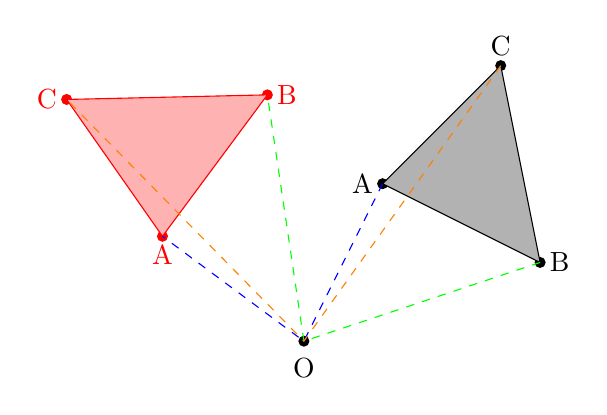
\begin{tikzpicture}
\coordinate (O) at (0,0);
\coordinate (A1) at (1,2);
\coordinate (B1) at (3,1);
\coordinate (C1) at (2.5,3.5);
\coordinate (A2) at ([rotate around={80:(0,0)}] 1,2);
\coordinate (B2) at ([rotate around={80:(0,0)}] 3,1);
\coordinate (C2) at ([rotate around={80:(0,0)}] 2.5,3.5);

\fill[black] (O) circle (2pt) node[below=1mm] {O};

\fill[black] (A1) circle (2pt) node[left] {A};
\fill[black] (B1) circle (2pt) node[right] {B};
\fill[black] (C1) circle (2pt) node[above] {C};
\fill[red] (A2) circle (2pt) node[below] {A};
\fill[red] (B2) circle (2pt) node[right] {B};
\fill[red] (C2) circle (2pt) node[left] {C};

\draw[black,fill=white!70!black] (A1)--(B1)--(C1)--cycle;
\draw[red,fill=white!70!red] (A2)--(B2)--(C2)--cycle;

\draw[dashed,blue] (A1)--(O)--(A2);
\draw[dashed,green] (B1)--(O)--(B2);
\draw[dashed,orange] (C1)--(O)--(C2);
\end{tikzpicture}

\begin{tikzpicture}
\coordinate (O) at (0,0);
\coordinate (A1) at (2,0.5);
\coordinate (B1) at (4,-0.5);
\coordinate (C1) at (3,3);
\coordinate (A2) at (-2,-0.5);
\coordinate (B2) at (-4,0.5);
\coordinate (C2) at (-3,-3);

\fill[magenta] (O) circle (2pt) node[xshift=7mm,yshift=-6mm] {対称の中心};

\fill[black] (A1) circle (2pt) node[below] {A};
\fill[black] (B1) circle (2pt) node[below] {B};
\fill[black] (C1) circle (2pt) node[above] {C};
\fill[red] (A2) circle (2pt) node[above] {A};
\fill[red] (B2) circle (2pt) node[above] {B};
\fill[red] (C2) circle (2pt) node[below] {C};

\draw[black,fill=white!70!black] (A1)--(B1)--(C1)--cycle;
\draw[red,fill=white!70!red] (A2)--(B2)--(C2)--cycle;

\draw[dashed,blue] (A1)--(O)--(A2);
\draw[dashed,green] (B1)--(O)--(B2);
\draw[dashed,orange] (C1)--(O)--(C2);
\end{tikzpicture}
\end{document}